%%%%%%%%%%%%%%%%%%%%%%%%%%%%%%%%%%%%%%%%%%%%%%%%%%%%%%%%%%%%%%%%%%%%%%%%
% FRONTPAGE
\newpage
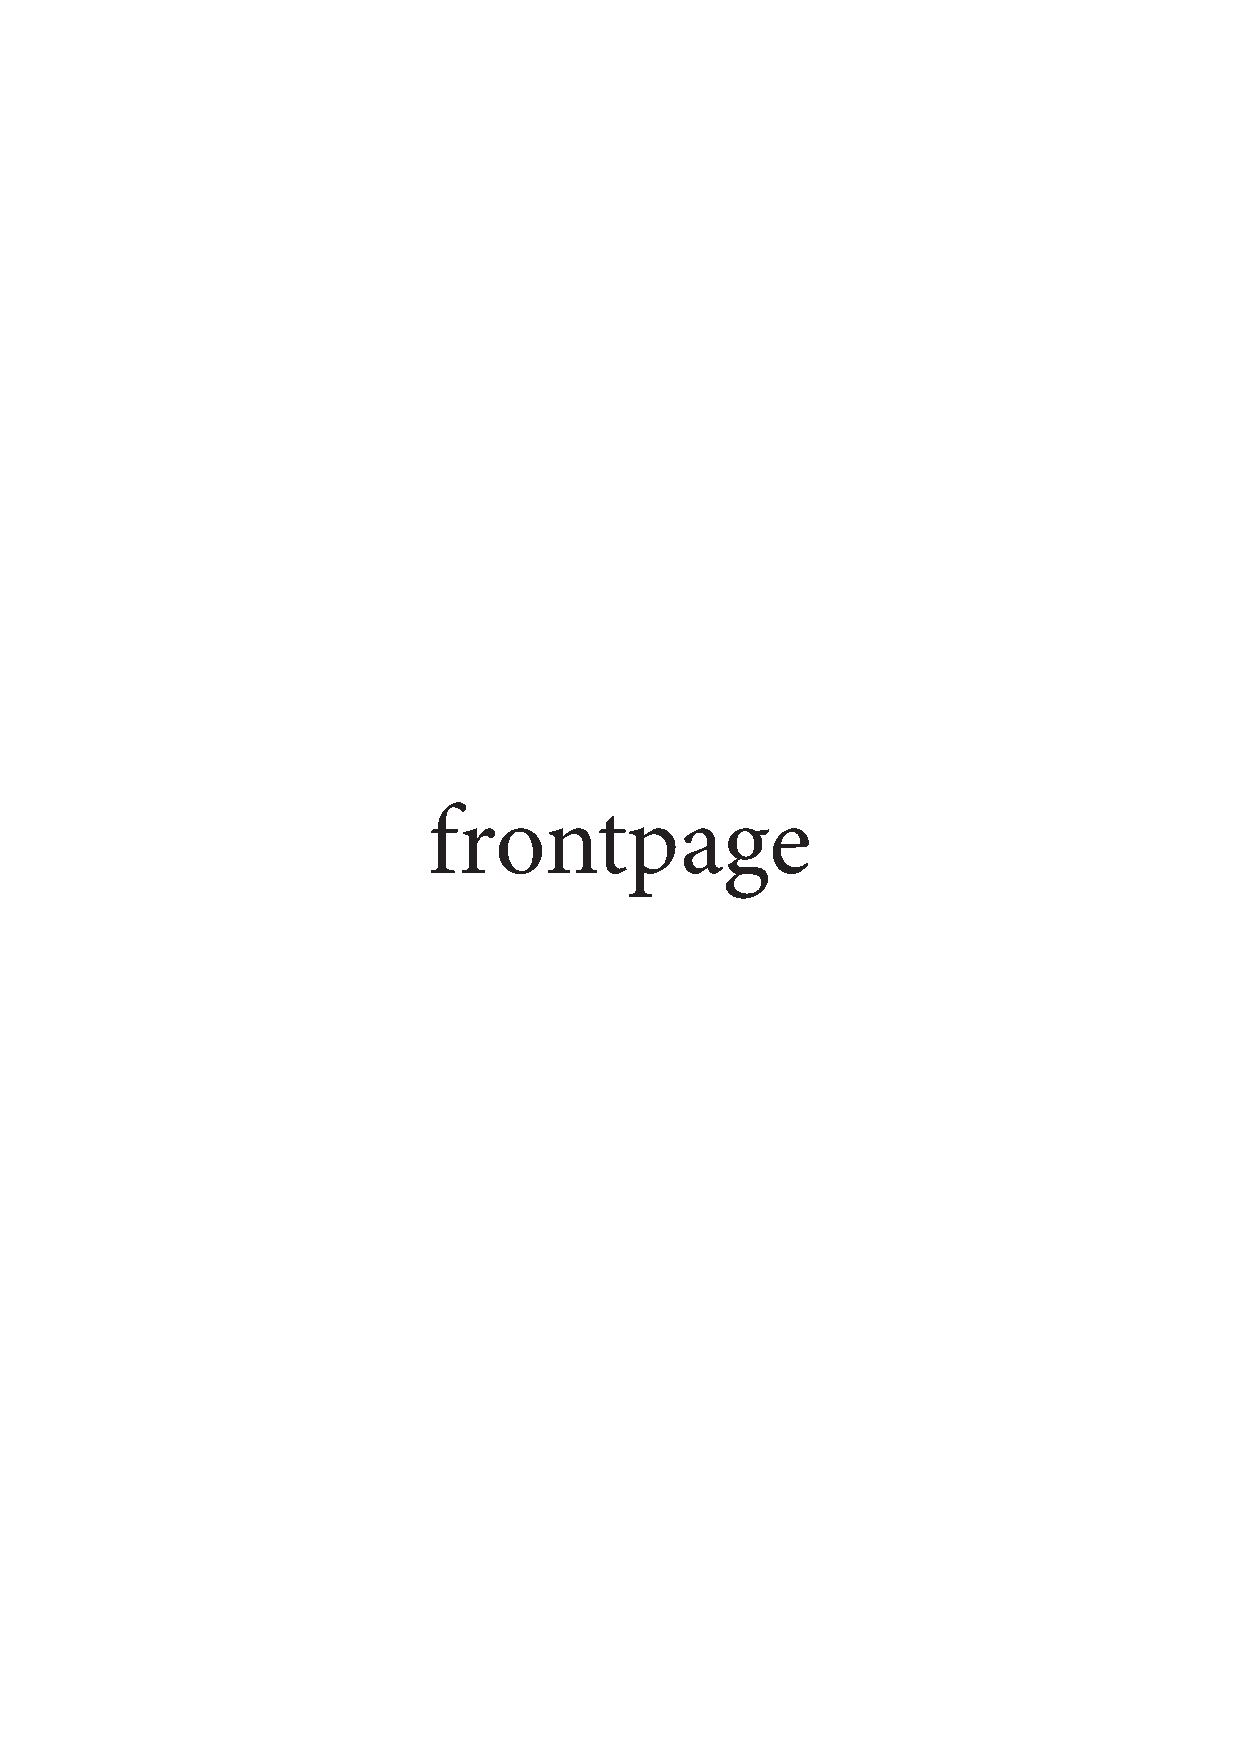
\includepdf[pages={1}]{documents/frontpage_placeholder.pdf} 
%replace your document

%%%%%%%%%%%%%%%%%%%%%%%%%%%%%%%%%%%%%%%%%%%%%%%%%%%%%%%%%%%%%%%%%%%%%%%%
% ASSIGNMENT
%\newpage
%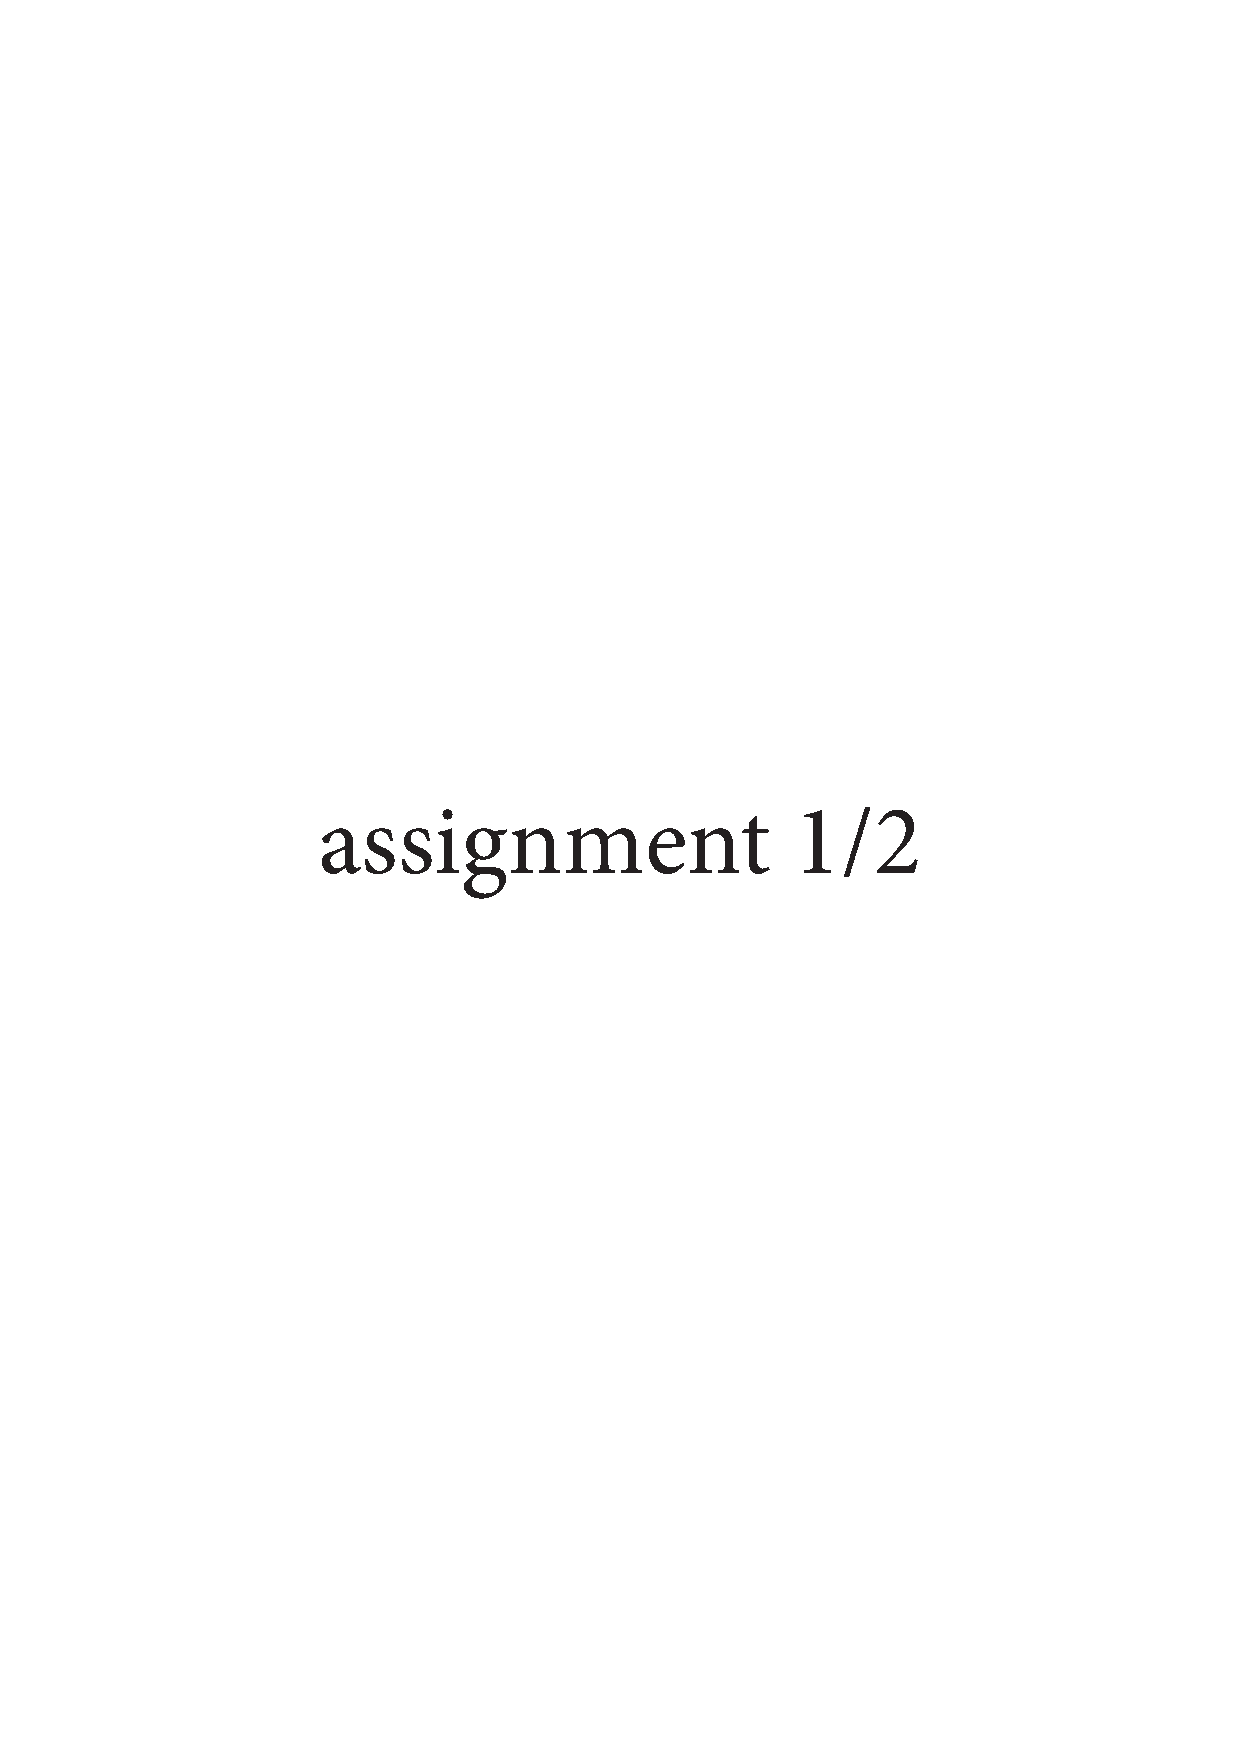
\includepdf[pages={1,2}]{documents/assignment_placeholder.pdf}
%replace your document

%%%%%%%%%%%%%%%%%%%%%%%%%%%%%%%%%%%%%%%%%%%%%%%%%%%%%%%%%%%%%%%%%%%%%%%%
% ACKNOWLEDGEMENT

\newpage
\thispagestyle{empty}

\vspace*{\fill}
\section*{ACKNOWLEDGEMENT}
\mbox
\indent I would like to very much thank my supervisor, Assoc. Ing. Ctirad Červinka, Ph.D. for his valuable advice on my way of learning the tools of computational chemistry, the opportunity to participate in real research and for the time devoted during consultations. Computational resources were provided by the e-INFRA CZ project (ID:90254), supported by the Ministry of Education, Youth and Sports of the Czech Republic.

%\vspace*{\fill}
% \noindent Práce byla podpořena projekty Grantové agentury ČR č. ...


%%%%%%%%%%%%%%%%%%%%%%%%%%%%%%%%%%%%%%%%%%%%%%%%%%%%%%%%%%%%%%%%%%%%%%%%

% SUMMARY

\newpage
\thispagestyle{empty}

\section*{SUMMARY}
Limited bioavailability of numerous active pharmaceutical ingredients is due to the poor solubility of their crystalline phases in water. Amorphous dispersions of drugs with biocompatible polymers offer a solution to overcome this issue, which currently impedes wider use of numerous drugs. This thesis will aim at molecular-dynamics modeling of binary systems containing selected poorly soluble active pharmaceutical ingredients and polylactic acid as a representative of biocompatible polymer excipients. Molecular dynamics simulations will be used to investigate the structural and cohesive properties of the neat substances and their mixtures with a special emphasis on analyzing the molecular interactions and compatibility between the drug and excipient molecules. An indispensable part of the thesis will be devoted to validate various simulation settings and to select an optimum setup for simulations of the bulk polymer in all atom resolution, taking aspects such as polymer chain length, polydispersity, thermal history and number of individual chains into account. Glass transition temperature and bulk phase densities will represent the main target properties for validation of the computational setup. Development of reliable computational models assessing the interactions of drugs with excipients will contribute to a rational design of novel drug formulations in the future.


\subsection*{keywords:}
\textit{Active pharmaceutical ingredients, Biocompatible polymer excipients, Amorphous solid dispersions, Glass transitions, Molecular dynamics}

%\bigskip %space between paragraphs
\newpage
\section*{SOUHRN}
Omezená biologická dostupnost mnoha aktivních farmaceutických látek se objevuje v důsledku špatné rozpustnosti jejich krystalických fází ve vodě. Příprava amorfních disperzí léčiv s biokompatibilními polymery nabízejí řešení k překonání tohoto problému, který v současnosti omezuje širší používání mnoha léčiv. Tato práce se zaměří na molekulárně-dynamické modelování binárních systémů obsahujících vybrané špatně rozpustné účinné farmaceutické složky a kyselinu polymléčnou jako zástupce biokompatibilních polymerních excipientů. Molekulárně-dynamické simulace budou použity ke zkoumání strukturních a kohezních vlastností čistých látek i jejich směsí se zvláštním důrazem na analýzu molekulárních interakcí a kompatibility mezi molekulami léčiva a pomocné látky. Nepostradatelná část práce bude zaměřena na ověření různých simulačních nastavení a výběru optimálního nastavení pro simulace polymeru v plném atomovém rozlišení, s přihlédnutím k hlediskům, jako je délka polymerního řetězce, polydisperzita, tepelná historie a počet jednotlivých řetězců. Teplota skelného přechodu a hustoty polymeru budou představovat hlavní cílové vlastnosti počítané pro validaci výpočetního nastavení. Vývoj spolehlivých výpočetních modelů hodnotících interakce léčiv s polymerními excipienty přispěje v budoucnu k racionálnímu návrhu nových lékových formulací.


\subsection*{klíčová slova:}
\textit{Farmaceuticky aktivní látky, Biokompatibilní polymerní excipienty, Amorfní pevné disperze, Skelný přechod, Molekulární dynamika}


% %%%%%%%%%%%%%%%%%%%%%%%%%%%%%%%%%%%%%%%%%%%%%%%%%%%%%%%%%%%%%%%%%%%%%%%%%
% Contents
\newpage
\thispagestyle{empty}
\tableofcontents

%deleting page numbering from all of the List of Contents pages
%\addtocontents{toc}{\protect\thispagestyle{empty}}
\addtocontents{toc}{\fontsize{4mm}{4mm}\selectfont\protect\enlargethispage{\baselineskip}}
\pagenumbering{gobble}